\begin{figure}[htbp]
	\centering
	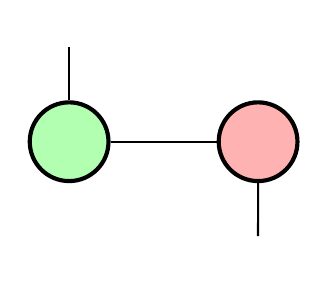
\begin{tikzpicture}[scale=1.2]
		\node[draw, circle, fill=green!30, minimum size=1cm, line width=1.5pt] (g1) at (0,0) {};
		\draw[thick] (g1) -- (0,1) node[above] {};
		\draw[thick] (g1) -- (2,0);

		\node[draw, circle, fill=red!30, minimum size=1cm, line width=1.5pt] (r1) at (2,0) {};
		\draw[thick] (r1) -- (2,-1) node[below] {};

	\end{tikzpicture}
	\caption{Bell state $|\Phi^+\rangle$ representation in the ZX calculus. The green spider represents the $|+\rangle$ state in the X basis, and connecting it to the red spider (in Z basis) creates the entangled Bell state. Bell state in ZX: A green spider with two outputs connected to a red spider with two inputs represents the maximally entangled Bell state $|\Phi^+\rangle = \frac{1}{\sqrt{2}}(|00\rangle + |11\rangle)$.}
	\label{fig:zx-bell-state}
\end{figure}
